\documentclass[11pt,a4paper]{article}

\usepackage[margin=1in, paperwidth=8.3in, paperheight=11.7in]{geometry}
\usepackage[ruled, vlined, linesnumbered]{algorithm2e}
\usepackage{amsfonts}
\usepackage{amsmath}
\usepackage{amssymb}
\usepackage{dsfont}
\usepackage{enumerate}
\usepackage{enumitem}
\usepackage{fancyhdr}
\usepackage{graphicx}
\usepackage{tikz}
\usepackage{changepage} 

\usepackage[utf8]{inputenc}
\usepackage{listings}
\usepackage{xcolor}

\lstset{
    frameround=fttt,
    language=Prolog,
    numbers=left,
    breaklines=true,
    mathescape=true,
    keywordstyle=\color{blue}\bfseries, 
    basicstyle=\ttfamily\color{red},
    numberstyle=\color{black}
    }

\begin{document}

\pagestyle{fancy}
\setlength\parindent{0pt}
\allowdisplaybreaks

\renewcommand{\headrulewidth}{0pt}
\setlist[enumerate,1]{label={\roman*)}}

% Cover page title
\title{Advanced Algorithms - Notes}
\author{Dom Hutchinson}
\date{\today}
\maketitle

% Header
\fancyhead[L]{Dom Hutchinson}
\fancyhead[C]{Advanced Algorithms - Notes}
\fancyhead[R]{\today}

% Counters
\newcounter{definition}[section]
\newcounter{example}[section]
\newcounter{notation}[section]
\newcounter{proposition}[section]
\newcounter{proof}[section]
\newcounter{remark}[section]
\newcounter{theorem}[section]

% commands
\newcommand{\dotprod}[0]{\boldsymbol{\cdot}}
\newcommand{\cosech}[0]{\mathrm{cosech}\ }
\newcommand{\cosec}[0]{\mathrm{cosec}\ }
\newcommand{\sech}[0]{\mathrm{sech}\ }
\newcommand{\prob}[0]{\mathbb{P}}
\newcommand{\nats}[0]{\mathbb{N}}
\newcommand{\cov}[0]{\mathrm{Cov}}
\newcommand{\var}[0]{\mathrm{Var}}
\newcommand{\expect}[0]{\mathbb{E}}
\newcommand{\reals}[0]{\mathbb{R}}
\newcommand{\integers}[0]{\mathbb{Z}}
\newcommand{\indicator}[0]{\mathds{1}}
\newcommand{\nb}[0]{\textit{N.B.} }
\newcommand{\ie}[0]{\textit{i.e.} }
\newcommand{\eg}[0]{\textit{e.g.} }
\newcommand{\X}[0]{\textbf{X}}
\newcommand{\x}[0]{\textbf{x}}
\newcommand{\iid}[0]{\overset{\text{iid}}{\sim}}
\newcommand{\proved}[0]{$\hfill\square$\\}
\newcommand{\Mod}[1]{\ \mathrm{mod}\ #1}

\newcommand{\definition}[1]{\stepcounter{definition} \textbf{Definition \arabic{section}.\arabic{definition}\ - }\textit{#1}\\}
\newcommand{\definitionn}[1]{\stepcounter{definition} \textbf{Definition \arabic{section}.\arabic{definition}\ - }\textit{#1}}
\newcommand{\proof}[1]{\stepcounter{proof} \textbf{Proof \arabic{section}.\arabic{proof}\ - }\textit{#1}\\}
\newcommand{\prooff}[1]{\stepcounter{proof} \textbf{Proof \arabic{section}.\arabic{proof}\ - }\textit{#1}}
\newcommand{\example}[1]{\stepcounter{example} \textbf{Example \arabic{section}.\arabic{example}\ - }\textit{#1}\\}
\newcommand{\examplee}[1]{\stepcounter{example} \textbf{Example \arabic{section}.\arabic{example}\ - }\textit{#1}}
\newcommand{\notation}[1]{\stepcounter{notation} \textbf{Notation \arabic{section}.\arabic{notation}\ - }\textit{#1}\\}
\newcommand{\notationn}[1]{\stepcounter{notation} \textbf{Notation \arabic{section}.\arabic{notation}\ - }\textit{#1}}
\newcommand{\proposition}[1]{\stepcounter{proposition} \textbf{Proposition \arabic{section}.\arabic{proposition}\ - }\textit{#1}\\}
\newcommand{\propositionn}[1]{\stepcounter{proposition} \textbf{Proposition \arabic{section}.\arabic{proposition}\ - }\textit{#1}}
\newcommand{\remark}[1]{\stepcounter{remark} \textbf{Remark \arabic{section}.\arabic{remark}\ - }\textit{#1}\\}
\newcommand{\remarkk}[1]{\stepcounter{remark} \textbf{Remark \arabic{section}.\arabic{remark}\ - }\textit{#1}}
\newcommand{\theorem}[1]{\stepcounter{theorem} \textbf{Theorem \arabic{section}.\arabic{theorem}\ - }\textit{#1}\\}
\newcommand{\theoremm}[1]{\stepcounter{theorem} \textbf{Theorem \arabic{section}.\arabic{theorem}\ - }\textit{#1}}

\tableofcontents

% Start of content
\newpage

\section{Hashing}

\definition{Dictionary}
A \textit{Dictionary} is an abstract data structure which stores $(\textit{key},\textit{value})$ pairs, with \textit{key} being unique.\\
A \textit{Dynamic Dictionary} can perform the following operations
\begin{center}
\begin{tabular}{l|l}
\textbf{Operation}&\textbf{Description}\\\hline
\lstinline!add(k,v)!&Add the pair \lstinline!(k,v)!.\\
\lstinline!lookup(k)!&Return \lstinline!v! if \lstinline!(k,v)! is in dictionary, \lstinline!NULL! otherwise.\\
\lstinline!delete(k)!&Remove pair \lstinline!(k,v)!, assuming \lstinline!(k,v)! is in dictionary.
\end{tabular}
\end{center}
A \textit{Static Dictionary} can only perform lookups, after it has been built.
\begin{center}
\begin{tabular}{l|l}
\textbf{Operation}&\textbf{Description}\\\hline
\lstinline!lookup(k)!&Return \lstinline!v! if \lstinline!(k,v)! is in dictionary, \lstinline!NULL! otherwise.
\end{tabular}
\end{center}

\proposition{Implementing a Dictionary}
Many data structures can be used to implement a \textit{Dictionary}.\\
These include, but not limited to:
\begin{enumerate}
	\item Linked lists.
	\item Binary Search, (2,3,4) \& Red-Black Trees.
	\item Skip lists
	\item van Emde Boas Trees.
\end{enumerate}

\remark{Motivation for Hashing}
None of the implementations of a \textit{Dictionary} suggested in \textbf{Proposition 1.1} achieves a $O(1)$ run-time complexity in the worst case for \underline{all} operations. To achieve this we introduce \textit{Hashing}.\\

\definition{Hash Function}
A \textit{Hash Function} takes in object's key and returns a value which is used to index the object in a \textit{Hash Table}.\\
Let $S$ be the set of all possible keys a hash function can recieve \& $m$ be the number of indexes in its \textit{Associated Hash Table}. Then
$$h:S\to[m]$$
\nb We want to avoid cases where $h(x)=h(y)$ for $x\neq y$(\textit{collisions}) .\\

\remark{Hashing functions assign items to indices with a geometric distribution}

\remark{Avoiding Collisions in Hashing}
When indexing $n$ items to $m$ indicies using a \textit{Hash Function} we only avoid \textit{Collisions} if $m\gg n$.\\

\definition{Hash Table}
A \textit{Hash Table} is an abstract data structre which extends the \textit{Dictionary} in such a way that time complexity is reduced.\\
A \textit{Hash Table} is comprise of an array \& a \textit{Hash Function}. The \textit{Hash Function} maps an object's key to an index in the array. If multiple objects have the same \textit{Hash Value} then a \textit{Linked List} is used in that index, with new objects added to the end of the \textit{Linked List} (Called \textit{Chaining}).\\

\proposition{Time Complexity for Dictionary Operations in a Hash Table}
By building a \textit{Hash Table} with \textit{Chaining} we achieve the following time complexities for \textit{Dictionary} operations
\begin{center}
\begin{tabular}{l|l|l}
\textbf{Operation}&\textbf{Worst Case Time Complexity}&Comments\\\hline
\lstinline!add(k,v)!&$O(1)$&Add item to the end of \textit{Linked List} if necessary.\\
\lstinline!lookup(k)!&$O($length of chain containing \lstinline!k!$)$&We might have to search through the whole\\&&\textit{Linked List} containing \lstinline!k!.\\
\lstinline!delete(k)!&$O($length of chain containing \lstinline!k!$)$&Only $O(1)$ to perform the actual deletion,\\
&&but need to find \lstinline!k! first.
\end{tabular}
\end{center}

\theorem{True Randomness}
Consider $n$ fixed inputs for a \textit{Hash Table} with $m$ indices. (\ie any sequence of $n$ \lstinline!add!/\lstinline!lookup!/\lstinline!delete! operations).\\
Pick a \textit{Hash Function}, $h$, at random from a set of all \textit{Hash Functions}, $H:=\{h:S\to[m])$. Then
$$\expect(\text{Run-Time per Operation})=O\left(1+\frac{n}{m}\right)$$
\nb The expected run-time per operation is $O(1)$ if $m\gg n$.\\

\proof{Theorem 1.1}
Let $x\ \&\ y\in S$ be two distincy keys \& $T$ be a \textit{Hash Table} with $m$ indexes.\\
Define $I_{x,y}\begin{cases}1&h(x)=h(y)\\0&\text{otherwise}\end{cases}$.\\
We have $\prob(h(x)=h(y))=\frac{1}{m}$.\\
Therefore
\[\begin{array}{rcl}
\expect(I_{x,y})&=&\prob(I_{x,y}=1)\\
&=&\prob(h(x)=h(y))\\
&=&\frac{1}{m}
\end{array}\]
Let $N_x$ be the number of keys stored in $H$ that are hashed to $h(x)$.\\
Note that $N_x=\displaystyle\sum_{k\in T}I_{x,k}$.\\
Now we have that
$$\expect(N_x)=\expect\left(\displaystyle\sum_{k\in T}I_{x,k}\right)=\sum_{k\in H}\expect(I_{x,k})=n\frac{1}{m}=\frac{n}{m}$$
\proved

\remark{Why not hash to unique values}
Suppose we want to define a \textit{Hash Function} which maps each key in $S$ to a unique position in the \textit{Hash Table}, $T$. This requires $m$ unique positions, which in turn require $\log_2 m$ bits for each key. This is an unreasonably large amount of space.\\

\proposition{Specifying the Hash Function}
Consider a set of \textit{Hash Functions}, $H:=\{h_1,h_2,\dots\}$.\\
When we initialise a \textit{Hash Table} we choose a hash function $h\in H$ at random and then proceed only to use $h$ when dealing with this specific \textit{Hash Table}.\\

\remark{Randomness in Hashing}
All the randomness in \textit{Hashing} comes from how we choose the \textit{Hash Function} \& not from how the \textit{Hash Function} itself runs.\\

\definition{Weakly Universal Set of Hashing Functions}
Let $H:=\{h|h:S\to[m]\}$ be a set of \textit{Hashing Functions}.\\
$H$ is \textit{Weakly Universal} if for any chosen $x,y\in S$ with $x\neq y$
$$\prob(h(x)=h(y))\leq\frac{1}{m}\text{ when varying }h(\cdot)$$
when $h$ is chosen uniformly at random from $H$.\\

\theorem{Expected Run time for Weakly Universal Set}
Consider $n$ fixeds to a \textit{Hash Table}, $T$, with $m$ indexes.\\
Pick a \textit{Hash Function}, $H$, from a \textit{Weakly Universal Set} of \textit{Hash Functions}, $H$.
$$\expect(\text{Run-Time per Operation})=O(1)\text{ for }m\geq n$$
\nb Proof is same as for \textit{True Randomness}.\\

\proposition{Constructing a Weakly Universal Set of Hash Functions}
Let $S:=[s]$ be the set of possible keys \& $p$ be some prime greater than $s$\footnote{There is a theorem that $\forall\ n\ \exists\ p\in[n,2n]$ st $p$ is prime.}.\\
Choose some $a,b\in[0,p-1]$ \& define
\[\begin{array}{rcl}
h_{a,b}(x)&=&\underbrace{[\ (ax+b)\Mod p\ ]}_\text{spread values over [0,p-1]}\underbrace{\Mod m}_\text{causes collisions}\\
H_{p,m}&=&\{h_{a,b}(\cdot):a\in[1,p-1],\ b\in[0,p-1]
\end{array}\]
\nb $H_{p,m}$ is a \textit{Weakly Universal Set} of \textit{Hashing Functions}.\\
\nb Different values of $a\ \&\ b$ perform differently for different data sets.\\

\remarkk{True Randomness vs Weakly Universal Hashing}
\begin{itemize}
	\item[-] For both \textit{True Randomness} \& \textit{Weakly Universal Hashing} we have that when $m\geq n$ the expected \lstinline!lookup! time in the \textit{Hash Table} is $O(1)$.
	\item[-] Constructing a \textit{Weakly Universal Set} of \textit{Hash Functions} is generally easier.
\end{itemize}

\theorem{Longest Chain - True Randomness}
If \textit{Hashing Function} $h$ is selected uniformly at random from all \textit{Hashing Functions} to $m$ indicies.\\
Then, over $m$ inputs we have
$$\prob(\exists\text{ a chain length}\geq3\log_2 m)\leq\frac1m$$

\proof{Theorem 1.3}
This problem is equivalent to showing that if we randomly throw $m$ balls into $m$ bins the probabiltiy of having a bin with at least $3\log_2 m$ balls is at most $\frac1m$.\\
Let $X_1$ be the number of valls in the first bin.\\
Choose any $k$ of the $M$ balls, the probabiltiy that all of these $K$ balls go into the first bin is $\frac1{m^k}$.\\
By the \textit{Union Bound Theorem} we have
$$\prob(X_1\geq k)\leq{m\choose k}\frac{1}{m^k}\leq1{k!}$$
Applying the \textit{Union Bound Theorem} again we have
$$\prob(\text{at least 1 bin recieves at least }k\text{ balls})\leq m\prob(X_1\geq k)\leq\frac{m}{k!}$$
Observe that
\[\begin{array}{rcl}
k!&>&2^{k-1}\\
\text{Let }k&=&3\log_2 m\\
\implies k!&>&2^{(3\log_2m-1)}\\
&\geq&2^{2\log_2 m}\\
&\geq&(2^{\log_2 m})^2\\
&=&m^2
\end{array}\]
Thus, setting $k=3\log_2 m$ means
$$\frac{m}{k!}\leq\frac1m\text{ for }m\geq2$$
\proved

\theorem{Longest Chain - Weakly Universal Hashing}
Let \textit{Hashing Function} $h$ be picked uniformly at random from a \textit{Weakly Universal Set} of \textit{Hashing Functions}.\\
Then, over $m$ inputs
$$\prob(\exists\text{ a chain length}\geq1+\sqrt{2m})\leq\frac12$$
\nb This is a poor bound.\\

\proof{Theorem 1.4}
Let $x,y\in S$ be two keys and define $I_{x,y}\begin{cases}1&h(x)=h(y)\\0&\text{otherwise}\end{cases}$.\\
Let $C$ be a random variable for the total number of collision (\ie $C=\sum_{x,y\in H, \x<y}I_{x,y}$).\\
Using \textit{Linearity of Expectation} and that $\expect(I_{x,y})=\frac1m$ when $h$ is \textit{Weakly Universal}
$$\expect(C)=\expect\left(\sum_{x,y\in H,\ x<y}I_{x,y}\right)=\sum_{x,y\in H,\ x<y}\expect(I_{x,y})={m\choose2}\frac1m\leq\frac{m}{2}$$
By \textit{Markov's Inequality}
$$\prob(C\geq m)\leq\frac{\expect(C)}m\leq\frac12$$
Let $L$ be a random variable for the length of the longest chain in $H$.\\
Then, $C\leq{L\choose2}$.
Now
$$\prob\left(\frac{(L-1)^2}{2}\geq m\right)\leq\prob\left({L\choose2}\geq m\right)\leq\prob(C\geq m)\leq\frac12$$
By rearranging, we have that
$$\prob(L\geq1+\sqrt{2m})\leq\frac12$$

\subsection{Perfect Hashing}

\remark{Motivation}
The \textit{Hashing Schemes} discussed in the previous part perform well in the best \& average cases but not necessarily in the worst cases (as they can have really long longest chains).\\

\definition{Static Perfect Hashing}
A \textit{Perfect Static Hashing Scheme} is a scheme that produces a \textit{Hash Table} where  \lstinline!lookup! has time complexity $\in O(1)$, even in the worst case. However this \textit{Hash Table} is static so we cannot perform \lstinline!insert! or \lstinline!delete! after the table has been produced.\\
\nb \textit{FKS Hashing Scheme} is a \textit{Perfect Static Hashing Scheme}.\\

\definition{FKS Hashing Scheme}
Below is an algorithm for the \textit{FKS Hashing Scheme}\\
\begin{algorithm}[H]
\SetKwInOut{Require}{require}
\caption{FKS Hashing Scheme}
\Require{$n \{\text{\# insertions}\}, T \{\text{Table with $n$ entries}\}$}
Insert all $n$ into $T$ using $h$\\
\While{Collisions in $T\geq n$}{
	Rebuild $T$ using a new $h$.
}
Let $n_i=|T[i]|$.\\
\For{$i\in[1,n]$}{
	Insert items of $T[i]$ into new table $T_i$ of size $n_i^2$ using $h_i$.\\
	\While{Collisions in $T_i\geq 1$}{
		Rebuild $T_i$ using a new $h_i$.
	}
}
\Return{T}
\end{algorithm}
\nb $\prob(\text{Collisions in }T_i\geq1)\leq\frac12$ and \nb $\prob(\text{Collisions in }T\geq n)\leq\frac12$ so we expect to have to build each table twice.\\

\remark{If $n$ items are mapped to the same index this counts as ${n\choose2}$ collision.}

\proposition{FKS Hashing Scheme - \lstinline!lookup!}
Below is an algorithm for \lstinline!lookup(x)! in the \textit{Hash Tables} produced by the \textit{FKS Hashing Scheme}
\begin{algorithm}[H]
\caption{FKS - \lstinline!lookup(x)!}
\SetKwInOut{Require}{require}
\Require{$T\ \{\text{main table}\}, \{T_1,\dots,T_m\}\ \{\text{sub-tables}\},x\ \{\text{key}\}$}
Compute $i=h(x)$.\\
Compute $j=h_i(x)$.\\
\Return{$T_i[j]$}
\end{algorithm}
\nb This runs in $O(1)$ time.\\

\proof{FKS Hashing Scheme - Space Requirements}
In the \textit{FKS Hashing Scheme} the main table $T$ requires space $O(n)$ and each sub-table $T_i$ requires space $O(n_i^2)$, where $n_i=|T[i]|$.\\
Storing each task function, $h_i$ requires space $O(1)$.\\
Thus the total space used is1
$$O(n)+\sum_iO(n_i^2)=O(n)+O\left(\sum_in_i^2\right)$$
We know there are ${n_i\choose 2}$ collisions in $T[i]$ so there are $\sum_i{n_i\choose 2}$ collisions in $T$.\\
We know there are at most $n$ collisions in $T$ so
$$\sum_i\frac{n_i^2}{4}\leq\sum_i{n_i\choose2}<n\implies\sum_in_i^2<4n$$
Thus
$$O(n)+O\left(\sum_in_i^2\right)=O(n)$$

\proof{FKS Hashing Scheme - Expected Construction Time}
The expected construction time for the main table, $T$, is $O(n)$.\\
The expected construction time for reach sub-table, $T_i$, is $O(n_i^2)$ where $n_i:=|T[i]|$.\\
Thus
\[\begin{array}{rcl}
expect(\text{construction time})&=&{\displaystyle\expect\left(\text{construction time of }T+\sum_i\text{construction time of }T_i\right)}\\
&=&\expect\text{construction time of }T)+{\displaystyle\expect\left(\sum_i\text{construction time of }T_i\right)}\\
&=&O(n)+{\displaystyle\sum_iO(n_i^2)}\\
&=&O(n)+{\displaystyle O\left(\sum_in_i^2\right)}\text{ see Proof 1.4}\\
&=&O(n)
\end{array}\]

\propositionn{FKS Hashing Scheme - Properties}
\begin{itemize}
	\item[-] Has no collisions.
	\item[-] \lstinline!lookup! takes $O(1)$ time in worst-case.
	\item[-] Uses $O(n)$ space.
	\item[-] Can be build in $O(n)$ expected time.
\end{itemize}

\subsection{Cuckoo Hashing}

%TODO something about bucketing
\remark{}
If our consruction has the property that $\forall\ x,y\in S$ with $x\neq y$ the probabiltiy that $x$ and $y$ are in the same bucket is $O\left(\frac1m\right)$, then for any $n$ operations the expected run-time is $O(1)$ per operation.\\

\definition{Cuckoo Hashing}
In \textit{Cuckoo Hasing} we use two hash functions, $h_1\ \&\ h_2$, to produce a single hash table.\\
When we \lstinline!add! a value $x$ to the hash table we place it in position $h_1(x)$. If there is already a value, $y$, already in this position then we move that value, $y$, to its alternative positione. We keep moving values until each value is in its position. If it is not possible (\ie we have found a cycle) then we change $h_1\ \&\ h_2$ for new hash functions and rehash all the values.\\
This is formally descibed in the algorithm below\\
\begin{algorithm}[H]
\SetKwInOut{Require}{require}
\caption{Cuckoo Hashing - Insert}
\Require{$\{x_1,\dots,x_n\}$ $\{\text{stream of keys}\}$, $T\ \{\text{Table with $m$ entries}\}$}
\textbf{choose} $h_1,h_2$
\For{$i\in[1,n]$}{
	$pos=h_1(x)$.\\
	$checked=[]$.\\
	\While{$T[pos]$ not empty}{
		\lIf{$x\in checked$}{\textbf{rehash}}
		$checked$ append $x$.
		$y=T[pos]$.\\
		$T[pos]=x$.\\
		$pos=$alternative position for $y$.\\
		$x=y$.
	}
	$T[pos]=x$.
}
\Return{T}
\end{algorithm}
\nb \textit{Rehash} involves chooseing two new hash functions $h_1\ \&\ h_2$ are reinserting all keys, $\{x_1,\dots,x_n\}$ into the table.\\

\propositionn{Cuckoo Hashing Scheme - Properties}
\begin{enumerate}
	\item An \lstinline!add! takes \textit{amortised exepcted} time $O(1)$.
	\item Every \lstinline!lookup! and every \lstinline!delete! has time complexity $O(1)$ in the worst-case.
	\item The space requirement is $O(n)$ where $n$ is the number of keys stored.
\end{enumerate}

\remark{Assumptions in Cuckoo Hashing}
In \textit{Cuckoo Hashing} we make the following assumptions
\begin{enumerate}
	\item $h_1$ and $h_2$ are indepenent.\\
	\ie $h_1(x)$ says nothing about $h_2(x)$, and visa-versa.
	\item $h_1$ and $h_2$ are truly random.\\
	\ie They map to each entry in the hash table with uniform probability.
	\item Computing the value of $h_1(x)$ and $h_2(x)$ takes $O(1)$ time in the worst-case.
\end{enumerate}

\definition{Cuckoo Graph}
A \textit{Cuckoo Graph} is an interprettation of a \textit{Hash Table} using \textit{Graph Theory}.\\
Each vertex of the graph is an entry in the hash table and for each $x_i$ we add an undirected-edge between $h_1(x_i)$ and $h_2(x_i)$.\\
If any cycles occur in a \textit{Cucko Graph} then we know construction will fail for that pair of hash functions as no stable scenario can occur.\\
The length of the longest path tells us the time for the longest insert.\\

\theorem{Probability of Long Paths in Cuckoo Graphs}
Let $m$ be the size of a hash table \& $n$ the number of entries we wish to insert
Fr any pair of positions $i$ and $j$, and any constant $c>1$, if $m\geq2cn$ then the probability that there exists a shortest path in the cuckoo graph from $i$ to $j$ with length $l\geq1$ is at most $\frac1{c^lm}$.\\

\proof{Theorem 1.5}
TODO\\

\proof{Probability of a path between two positions in a Cuckoo Graph}
If a path exists from $i$ to $j$, ther emust be a shortest path from $i$ to $j$.\\
Therefore we can use \textbf{Theorem 1.5} and the \textit{Union Bound} over all possible paths to show the probability of a path from $i$ to $j$ existing is at most
$$\sum_{l=1}^\infty\frac1{c^lm}=\frac1m\sum_{l=1}^\infty\frac1{c^l}=\frac1m\frac1{c-1}=O\left(\frac1m\right)$$

\definition{Buckets}
We say that two keys $x\ \&\ y$ are in the same \textit{bucket} iff there exists a path from $h_1(x)$ to $h_1(y)$ in a \textit{Cuckoo Graph}.\\
Note that this implies there is a path from $h_1(x),h_2(y)$; $h_2(x),h_1(y)$ and $h_2(x),h_2(y)$ as there are edges $(h_1(x),h_2(x))$ \& $(h_1(y),h_2(y))$.\\

\remark{The time for an operation on $x$ is bounded by the number of items in its bucket.}

\proposition{Probabiltiy of being in the same Bucket}
For $x,y\in S$ with $x\neq y$ the probability that they are in the same bucket is at most
$$\sum_{l=1}^\infty\frac1{c^lm}=\frac1m\sum_{l=1}^\infty\frac1{c^l}=\frac1m\frac1{c-1}=O\left(\frac1m\right)$$
If the size of a hash table is $m\geq2cn$ then the expeceted time per operation is $O(1)$.\\
Further, \lstinline!lookup!s take $O(1)$ time in the worst case.\\

\proposition{Probability of Rehashing}
The probabiltiy that a rehashing occurs in \textit{Cuckoo Hashing} is equal to the probability of the \textit{Cuckoo Graph} having a cycle.\\
A cycle is a path from $x$ to $x$, via some intermidiary vertices.\\
Thus the probability that $x$ is involved in a cycle is
$$\sum_{l=1}^\infty\frac1{c^lm}=\frac1{m(c-1)}$$
by \textbf{Proof 1.7}.\\
Thus the probabiltiy that there is at least one cycle in the whole hash table is
$$m\frac1{m(c-1)}=\frac1{c-1}$$

\proposition{Construction Time - Cuckoo Hashing}
Consider the result in \textbf{Proposition 1.9} when $c=3$.\\
The probability of a rehashing occuring is $\frac12$.\\
Thus we expected only one rehash to be necessary. The the expected time for a rehash is $O(n)$ then the expeceted construction time for the table is $O(n)$.\\
Therefore the \textit{amortised expeced} time for rehashes over $n$ insertions is $O(1)$ per insertion.\\
\nb Checking for a cycle in a graph takes $O(n)$ time.

\section{Bloom Filters}

\definition{Bloom Filter}
A \textit{Bloom Filter} is a data structure which is designed to be a space efficient way of storing a set $S$.\\
\textit{Bloom Filters} support only the following operations
\begin{center}
\begin{tabular}{l|l}
\textbf{Operation}&\textbf{Description}\\\hline
\lstinline!insert(k)!&Insert the key \lstinline!(k)!.\\
\lstinline!member(k)!&Returns \lstinline!true! if \lstinline!(k)!$\in S$, no otherwise.
\end{tabular}
\end{center}
Note that there is no way to remove objects from a \textit{Bloom Filter} \& you cannot ask which keys are in the \textit{Bloom Filter}, only whether a particular key is.\\
\nb \textit{Bloom Filters} are meant to be used in cases where the size of the sample space is much larger than the number of keys being stored.\\

\remark{Motivation}
\textit{Bloom Filters} can be used to build a blacklist of unsafe URLS. Whenever a new unsafe URL, \lstinline!k!, is discovered we add it to the filter, \lstinline!insert(k)!.\\
Whenever we want to visit to a new URL, \lstinline!k!, we can query whether it is in the bloom filter, \lstinline!member(k)!, and if we are returned \textit{yes} then it is blocked.\\

\remark{Randomness in Bloom Filter}
A \textit{Bloom Filter} is randomised in such a way that \lstinline!member(k)! will sometimes return \textit{yes} when in fact \lstinline!k!$\not\in S$. However it will never return \textit{no} if \lstinline!k!$\in S$.\\
\nb The amount of space used by a \textit{Bloom Filter} depends on the failure rate we allow it.\\

\proposition{Usefullness of Bloom Filter}
For a \textit{Bloom Filter} \lstinline!insert(k)! \& \lstinline!member(k)! both run in $O(1)$ and it requries $O(n)$ bits of space to store up to $n$ keys.\\

\proposition{Building a Bloom Filter - Array}
A na\"ive approach to building a \textit{Bloom Filter} is to use an array.\\
Suppose we have sample space $1,2,\dots,|U|$ for key values.\\
We can store a set by mainting a bit string $B$ where $B[k]=1$ if $k\in S$ and $B[k]=0$ otherwise.\\
\eg \begin{tabular}{|c|c|c|c|c|c|}
\hline
1&2&3&4&5&6\\\hline
0&1&0&0&0&1\\\hline
\end{tabular} here $|U|=6$ and $S=\{2,6\}$.\\
The \textit{Bloom Filter} operations take $O(1)$ time but the array is $|U|$ long.\\

\proposition{Building a Bloom Filter - Hash Table}
Let $h:U\to[1,m]$ be a hash function.\\
We can implement a \textit{Bloom Filter} using a \textit{Hash Table} is we define that performing \lstinline!insert(k)! sets $B[h(k)]=1$ and \lstinline!member(k)! returns $\mathtt{true}$ if $B[h(k)]==1$, and $\mathtt{false}$ otherwise.\\
Using a hash function means the bit string $B$ being maintained is much shorter than if we used the \textit{Array} approach in \textbf{Proposition 2.2}, however we now have to deal with collisions \& thus false-positive results from \lstinline!member(k)!.\\
\nb false-positives occur \lstinline!member(k)! if $\exists k'\in S$ st $h(k')=h(k)$.\\

\remark{Reducing Collisions - Bloom Filter as Hash Table}
To ensure a low probability of collisions each operation, we pick the hash function $h$ at random (Note that we don't change $h$ after it is set).\\

\proposition{Probability of False Positive - Bloom Filter as Hash Table}
Suppose we have inserted $n$ keys into the \textit{Bloom Filter} and now we perform \lstinline!member(k)! for $k\not\in S$.\\
The bit string $B$ contains at most $n$ 1s among its $m$ positions.\\
By definition the hash function assigns values uniformly $\prob(h(i)=j)=\frac1m$ for $k\in[1,m]$.\\
Thus the probability of a false-positive is $\prob(B[h(k)]=1)\leq\frac{n}m$.\\
If we choose $m$ to be $100n$ then $\prob(B[h(k)]=1)\leq.01$.\\

\proposition{Bloom Filter Complexities}
Both \lstinline!insert(k)! and \lstinline!member(k)! run in $O(1)$ and the structure uses $m$ bits.\\
If we want a .01 false positive rate then $100n$ bits are required.\\

\proposition{Building a Bloom Filter - Proper}
Again we are maintaining a bit string $B$ of length $m<|U|$.\\
Let $h_1,\dots,h_r$ be $r$ hash functions which map $U\to[1,m]$ uniformly at random.
\begin{itemize}
	\item[-] \lstinline!insert(k)! sets $B[h_i(k)]=1$ for \underline{all} $i\in[1,r]$.
	\item[-] \lstinline!member(k)! returns $\mathtt{true}$ iff $B[h_i(k)]=1\ \forall\ i\in[1,r]$.
\end{itemize}

\proposition{Probability of False Positive for \textbf{Proposition 2.6}}
Assume that we have inserted $n$ keys into the \textit{Bloom Filter} and that we are performing \lstinline!member(k)! for $k\not\in S$.\\
This checks whether $B[h_i(k)]=1\ \forall\ i\in[1,r]$.\\
This is question whether $r$ randomly chosen bits of $B$ all equal 1 due to hash functions being uniformly random.\\
As there are $n$ keys in the \textit{Bloom Filter} at most $nr$ bits of $B$ are set to 1.\\
So $\frac{nr}{m}$ is the proportion of bits set to $1$ in $B$.\\
So the probability that a ranomly chosen bit is $1$ is $\leq\dfrac{nr}{m}$.\\
Thus the probability that $r$ randomly chosen bits are all equal to 1 is $\leq\left(\dfrac{nr}{m}\right)^r$.\\

\proposition{Minimising False Positive Rate}
By differentiating $\leq\left(\dfrac{nr}{m}\right)^r$ we find it is minimised for $r=\frac{m}{ne}$.\\
If we substitute this back in we get a false positive rate of at most $\left(\frac1e\right)^{\frac{m}{ne}}\approx(0.69)^\frac{m}{n}$.\\
So for a failure rate of $1\%$ we set $m\approx12.52 n$.\\
This is much better than $m=100n$ required for \textbf{Proposition 2.4}.\\

\remark{Limitations of Hashing}
Using \textit{Hashing} for dynamic dictionaries has a few draw backs
\begin{enumerate}
	\item Randomness.
	\item Amortisation, \ie expected complexities are averaged over $n$.
	\item Inflexible, hard to add new operations.
\end{enumerate}

\section{van Emde Boas Trees}

\proposition{New operations for Dynamic Dictionary}
Below are some operations which are often used as an extension to the \textit{Dynamic Dictionary} in \textbf{Definition 1.1}.
\begin{center}
\begin{tabular}{l|l}
\textbf{Operation}&\textbf{Description}\\\hline
\lstinline!predecessor(k)!&Return the pair \lstinline!(x,v)! in the dictionary\\
&with the largest key,  \lstinline!x!, such that \lstinline!x!$\leq$\lstinline!k!.\\
\lstinline!successor(k)!&Return the pair \lstinline!(x,v)! in the dictionary\\
&with the smallest key,  \lstinline!x!, such that \lstinline!x!$\geq$\lstinline!k!.\\
\end{tabular}
\end{center}
\nb \textit{Hashing}-based dynamic dictionaries are not suited to these operations.\\

\proposition{Implementing New Operations}
We could use self-balancing binary trees such as \textit{2-3-4 Trees}, \textit{Red-Black Trees} or \textit{AVL Trees}.\\
These can perform all five operations of our extended dynamic dictionary each in $O(\log n)$ worst case time and $O(n)$ space.\\

\definition{Van Emde Boas Trees}
\textit{Van Emde Boas Trees} can support the five operations of our \textit{Extended Dynamic Dictionary}.\\
\textit{Van Emde Boas Trees} can perform each operation in $O(\log\log u)$ time and use $O(u)$ space where $u$ is the size of the universe.\\
\nb Also known as \textit{vEB Trees}.\\

\proposition{vEB Trees - Array}
Suppose we wishing to store the set $S\subset U$ keys with $u=|U|$.\\
Let $A$ be a binary array of size $u$ where $A[i]=1$ iff $i\in S$.\\
We can use the following schema for each operation of the \textit{Extended Dynamic Dictionary}
\begin{enumerate}
	\item \lstinline!add(x)! - Set $A[x]=1$.
	\item \lstinline!delete(x)! - Set $A[x]=0$.
	\item \lstinline!lookup(x)! - Return $\mathtt{true}$ if  $A[x]=1$, $\mathtt{false}$ otherwise.
	\item \lstinline!predecessor(x)! - Increase $i$ until \lstinline!lookup(x-i)! returns $\mathtt{true}$. Return $x-i$.
	\item \lstinline!successor(x)! - Increase $i$ until \lstinline!lookup(x+i)! returns $\mathtt{true}$. Return $x+i$.
\end{enumerate}
Here \lstinline!add!, \lstinline!delete! \& \lstinline!lookup! take $O(1)$ time, but \lstinline!predecessor! \& \lstinline!successor! take $O(u)$ time. (Not great).\\

\proposition{vEB Trees - Blocks}
Let $S\subset U$ where $U$ is a universe of size $u$.\\
Let $B_1,\dots,B_{\sqrt{u}}$ be bit vectors of length $\sqrt{u}$ which define sequential blocks of $U$.\\
Each of these vectors stores the values $\{0,\dots,\sqrt{u}-1\}$. $B_i[j]\equiv1$ iff $x:=j+\sqrt{u}\cdot i$ is in $S$.\\
Let $C$ be a bit vector of length $\sqrt{u}$ which summaries the blocks $B_1,\dots,B_{\sqrt{u}}$.\\
We have that $C[i]\equiv1$ iff block $B_i$ is non-empty.\\
With this set up be can fulfil the oeprations as follows
\begin{itemize}
	\item[\lstinline!add(x)!]
	\begin{enumerate}
		\item Define $i:=\lfloor x/\sqrt{u}\rfloor$ \& $j:=x-i\cdot\sqrt{u}$.
		\item Set $B_i[j]=1$ \& $C[i]=1$.
	\end{enumerate}
	\item[\lstinline!delete(x)!]
	\begin{enumerate}
		\item Define $i:=\lfloor x/\sqrt{u}\rfloor$ \& $j:=x-i\cdot\sqrt{u}$.
		\item Set $B_i[j]=0$.
		\item Check if $B_i$ is empty. If so set $C[i]=0$.
	\end{enumerate}
	\item[\lstinline!successor(x)!]
	\begin{enumerate}
		\item Define $i:=\lfloor x/\sqrt{u}\rfloor$ \& $j:=x-i\cdot\sqrt{u}$.
		\item Look for successor to $x$ in $B_i$, starting at $B_i[j]$.
		\item If no successor exists
		\begin{enumerate}
			\item Find succesor to $j$ in $C$, starting at $C[j+1]$.
			\item Return smallest element in that block.
		\end{enumerate}
	\end{enumerate}
\end{itemize}
\nb In practive the blocks are implemented as a single bit-vector.\\

\remark{\lstinline!successor(x)! for Blocks Implementation}
In the block implementation of \textit{vEB Trees} we have $T(u)=3T(\sqrt{u})+O(1)$ as we make 3 recursive calls to \lstinline!successor()!.\\
This gives time complexity $T(u)\in O(\sqrt{u})$.\\
We can improve this by reducing the number of recursive calls made.\\
To do this we restructure the data structure. (See \textbf{Proposition 3.5}).\\

\proposition{vEB Trees - Proper}
Consider the same set up as in \textbf{Proposition 3.4}.\\
Here the data structure is augment such that for each block $B_i$ we store the $\mathtt{max}$ and $\mathtt{min}$ indexes used in it.\\
By doing this we can perform \lstinline!successor(x)! as follows
\begin{enumerate}
	\item Define $i:=\lfloor x/\sqrt{u}\rfloor$ \& $j:=x-i\cdot\sqrt{u}$.
	\item If $j>\mathtt{max}_i$: \# No successor in block
	\begin{enumerate}
		\item $k=$\lstinline!$\text{successor}_C(i)$! \# Find block with next value
		\item return $B_k[\mathtt{min}_k]$
	\end{enumerate}
	\item Else: \# Successor is in block
	\begin{enumerate}
		\item return \lstinline!$\text{successor}_{B_i}(j)$!
	\end{enumerate}
\end{enumerate}
We are now only ever making a single recurisve call, giving us $T(u)=T(\sqrt{u})+O(1)$.\\
Thus $T(u)\in O(\log\log u)$.\\
\nb Each block \& summary can be defined recursively.\\

\example{vEB Trees - Proper}
Consider a universe of size $u=16$.\\
The following is an example of the datat structure that would be used
$$C=\begin{pmatrix}1\\0\\0\\1\end{pmatrix}\quad B=\begin{pmatrix}1&0&0&0\\0&0&0&0\\0&0&0&0\\0&1&0&1\end{pmatrix}\quad\mathtt{min}=\begin{pmatrix}0\\-\\-\\1\end{pmatrix}\quad\mathtt{max}=\begin{pmatrix}0\\-\\-\\3\end{pmatrix}$$
\nb Each row relates to a single block.\\

\remark{Time Complexity of \lstinline!add! for vEB Trees}
\lstinline!add! contain a single recursive call.\\
We have that $T(u)=T(\sqrt{u})+O(1)$.\\
By the Master's Theorem we have that $T(u)=O(\log\log u)$.\\
\nb This is the same for all operations.\\


\remark{Space Complexity of vEB Trees}
Let $Z(u)$ be the space use by a \textit{vEB Tree} over a universe of size $u$.\\
We have that
$$Z(u)=(\sqrt{u}+1)Z(\sqrt{u})+O(1)\implies Z(u)=O(u)$$

\section{Orthogonal Range Searching}

\definition{$nD$ Range Searching Data Structure}
An \textit{$n$-Dimensional Range Searching Data Structure} stores $m$ distinct $n$-dimensional data points and supports a single operation
\begin{center}
\begin{tabular}{l|l}
\textbf{Operation}&\textbf{Description}\\\hline
\lstinline!lookup($l_1,u_1,\dots,l_1,u_1$)!&Return all stored points $(z_1,\dots,z_n)$ where\\
&$l_1\leq z_1\leq u_1$ and $\dots$ and $l_n\leq z_n\leq u_n$.
\end{tabular}
\end{center}

\proposition{$1D$ Range Searching Data Structure}
Consider an array of stored values $[x_1,\dots,x_n]$.\\
Make a balanced binary tree by recursively taking the midpoint of the array as a new node and then partitioning the values around.\\
\lstinline!lookup($l_1,u_1$)! can be performed as follows
\begin{enumerate}
	\item Find the successor of $l_1$. Takes $O(\log n)$ time.
	\item Find the predecessor of $u_1$. Takes $O(\log n)$ time.
	\item Find the path between the successor and predecessor.
	\item For each node on path:
	\begin{enumerate}
		\item Consider its left \& right subtree in turn (if they exist).
		\item If root of subtree is in $[l_1,u_1]$ then return all values in subtree.
	\end{enumerate}
\end{enumerate}
This implementation of \lstinline!lookup($l_1,u_1$)! takes $O(\log n+k)$ time, where $k$ is the number of points to be returned, and $O(n)$ space and $O(n\log n)$ prep-time (to construct the tree).\\
\nb Runtime depends on the size of the output.\\

\proposition{$2D$ Range Searching Data Structure - Na\"ive}
Below is a na\"ive approach for performing \lstinline!lookup(lx,ux,ly,uy)!
\begin{enumerate}
	\item Find all the points with $l_x\leq x\leq u_x$ using \textbf{Proposition 4.1}.
	\item Find all the points with $l_y\leq y\leq u_y$.
	\item Find the points in both lists.
\end{enumerate}
This approach has run time $O(\log n+k_x)+O(\log n+k_y)+O(k_x+k_y)=O(n+k_x+k_y)$ where $k_x$ is the number of points found in step $i)$ and $k_y$ is the number of points found in step $ii)$.\\

\proposition{$2D$ Range Searching Data Structure - Proper}
For preprocessing build a balanced binary tree using the $x$ value of each point.\\
Here is a better implementation of \lstinline!lookup($1_x,u_x,l_y,u_y$)!.
\begin{enumerate}
	\item Find the successor to $l_x$.
	\item Find the predeccessor to $u_x$.
	\item Find the path between these two points.\\
	Each subtree on this path has the property that either \underline{all} points in the tree have $x$ values in the range $[l_x,u_x]$, or \underline{none} of them do.
	\item For each subtree where \underline{all} points have $x$ values in the range $[l_x,u_x]$.
	\begin{enumerate}
		\item Build a \textit{1D Range Searching Structure} using the $y$-coordinates of each point in the tree.
		\item Perform \lstinline!lookup($l_y,u_y$)! on this subtree.
	\end{enumerate}
\end{enumerate}

\remark{Time Complexity \textbf{Proposition 4.3}}
Steps $i)-iii)$ take $O(\log n)$ time and the length of the path between the successor \& predecessor is of length $O(\log n)$.\\
In step $iv)$ we do $O(\log n)$ 1-D lookups. Each of these takes $O(\log n+k')$ time.\\
Thus the overall run-time is $O(log^2n+k)$ as each lookup is disjoint.\\
\nb Preprocessing takes $O(n\log n)$ time.\\

\remark{Space Complexity \textbf{Proposition 4.3}}
The initial 1D structure used $O(n)$ space.\\
At each node we stored an array containing the points in its subtree.\\
The tree has depth $O(\log n)$.\\
Thus the total space used is $O(n\log n)$.

\section{Pattern Matching}

\definition{Exact Pattern Matching Problem}
Let $T,P$ be strings of length $n,m$ respectively.\\
The \textit{Exact Pattern Matching Problem} is to find all occurences of $P$ in $T$.\\
$P$ matches at location $i$ iff $\forall\ j\in[0,m)\ P[j]=T[i+j]$.

\proposition{Na\"ive Algorithm}
A \textit{Na\"ive Algorithm} for solving the \textit{Exact Pattern Matching Problem} is to align $P$ with the start of $T$; compare every character; return if a match has occured; slide on by one character; repeat until end of $T$ is reached.\\
\nb This takes $O(nm)$ time.\\

\proposition{Proper Algorithms}
Proper Algorithms can solve the \textit{Exact Pattern Matching Problem} (\eg KMP) in $O(n)$ time.\\
Note that this mean run times depends on the size of the text being analysed, not on the pattern which is being searched for.\\

\remark{Preprocessing}
Since the text, $T$, is constant across all queries, it is acceptable to do a significant amount of preprocessing in order to speed up query times.

\subsection{Suffix Trees}

\definition{Suffix}
A \textit{Suffix} is any substring of a string which includes the last character.\\

\definition{Atomic Suffix Tree}
An \textit{Atomic Suffix Tree} is a tree where each edge is a labled by a character \& each leaf is labelled with the index at which a given suffix starts.\\
Each root-to-leaf path is a suffix in the tree.\\

\example{Atomic Suffix Tree}
Below is an \textit{Atomic Suffix Tree} for `bananas'.
\begin{center}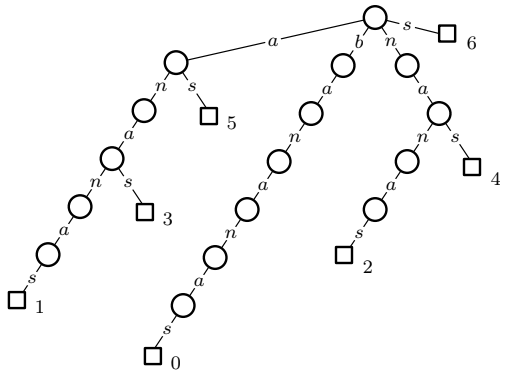
\includegraphics[scale=.5]{img/atomic_suffix_tree.png}\end{center}

\proposition{Searching a Atomic Suffix Tree}
We can use an \textit{Atomic Suffix Tree} to solve the \textit{Exact Pattern Matching Problem}.\\
Given an pattern $P$, starting at the root, step down the path dictated by $P$.\\
If $P$ requires a step which cannot be fulfilled then that pattern does not exist anywhere in $T$.\\
If the path of $P$ does terminate successfully on a node: return all the leaf values in this nodes subtree.\\

\remark{Runtime}
This approach has runtime complexity of $O(m)$.\\
It should be noted that the number of choices we have to check at each node does affect the runtime, however for constant size alphabets this is not of great concern.\\

\remark{Limitations of Atomic Suffix Tree}
\textit{Suffix Trees} can have upto $\left(\frac{n}2+1\right)^2$ internal nodes, meaning its space requirements are $O(n^2)$ are quickly become unmanageable.\\
They can contain long paths.\\

\definition{Compacted Suffix Tree}
A \textit{Compacted Suffix Tree} has the same structure as an \textit{Atomic Suffix Tree}, the only difference being that any non-branching nodes (\ie nodes with only one child) are merged into the node below and edges are now labelled with Substrings.\\
This means that every node has at least $2$ children and we have $O(n)$ edges.\\
\nb In practice we do not store the substring for each edge but rather the endpoints in $T$ in order to save space.\\

\example{Compact Suffix Tree}
Below is an \textit{Compact Suffix Tree} for `bananas'.
\begin{center}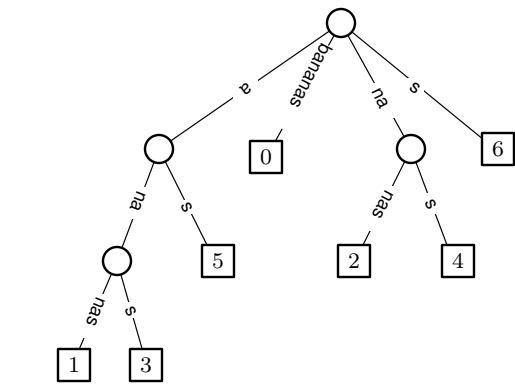
\includegraphics[scale=.5]{img/compact_suffix_tree.png}\end{center}

\proposition{A Compact Suffix Tree does \textbf{not} always exist}
A complete \textit{Compact Suffix Tree} does not always exist.\\
Suppose $T=$`$bb$' then the tree would contain a single edge and we would not successfully detect the pattern $P=$`$b$'.\\
This can be fixed by adding a character which does not appear in $T$ onto the end (\eg $T=$`$bb\$$').

\proposition{Searching a Compact Suffix Tree}
Same process as for an \textit{Aromic Suffix Tree} except we are comparing multiple characters at a time.\\
Run time is $O(m+\#\text{occurences})$.\\

\propositionn{Constructing a Compact Suffix Tree - Na\"ive}
\begin{enumerate}
	\item Insert the suffixes one at a time, longest to shortest:
	\begin{enumerate}
		\item Search for the new suffix in the partial suffix tree.\\
		(Same technique as pattern matching).
		\item Add a new edge and leaf for the new suffix.\\
		This may require the breaking of an edge into two.
	\end{enumerate}
\end{enumerate}
This has run-time complexity $O(n^2)$.\\
\nb This can be done in $O(n)$ time but is not covered on this course.\\

\proposition{Multiples Texts}
If we want to be able to search multiple texts we a character to the end of each text: this characters must be different \& not appear in any of the texts.\\
We then append these texts and treat them as a single text.

\subsection{Suffix Arrays}

\definition{Lexicographical Sorting}
\textit{Lexicographical Sorting} is a way of ordering words in alphabetical order.\\
Let $T_1$ and $T_2$ be two texts which we are sorting.
\begin{itemize}
	\item Compare $T_1$ \& $T_2$ character-by-character.
	\item Let $i$ be the index of the first character to differ between $T_1$ \& $T_2$.
	\item If $T_1[i]<T_2[i]$ alphabetically (or any order defined ordering) then $T_1$ is placed first, and visa-versa.
	\item If no characters differ but $T_1$ is shorter than $T_2$, then $T_1$ is placed first and visa-versa.
\end{itemize}
\nb This is how words are sorted in the dictionary.\\

\definition{Suffix Array}
Let $T$ be a text with $|T|=n$.\\
Lexicographic sort all $n$ suffices of $T$.\\
We define a \textit{Suffix Array}, $A$, st
$$A[i]=n-\text{length of suffix with was }i^\text{th}\text{ in lexicographic order}$$

\example{Suffix Array}
Consider the word \textit{`bananas'}.
\begin{center}
\begin{tabular}{|r|l|}
\hline
$n-l$&\textbf{suffix}\\\hline
0&bananas\\
1&ananas\\
2&nanas\\
3&anas\\
4&nas\\
5&as\\
6&s\\
\hline
\end{tabular}\quad
\begin{tabular}{|r|l|}
\hline
$n-l$&\textbf{suffix}\\\hline
\hline
1&ananas\\
3&anas\\
5&as\\
0&bananas\\
2&nanas\\
4&nas\\
6&s\\
\hline
\end{tabular}
\end{center}
Thus, in this case, $A=[1,3,5,0,2,4,6]$.\\

\remark{Suffix arrays are much smaller than Suffix Trees}

\proposition{Suffix Array from Suffix Tree}
If we already have a \textit{Suffix Tree} constructed then we can construct a \textit{Suffix Array} by performing a depth first search on the tree and setting $A[i]$ to be the $i^\text{th}$ element to be returned by this search.\\
\nb Depth first search can be done in $O(n)$ time.\\

\proposition{Searching a Suffix Array}
Let $T$ be a text we wish to search and $P$ be the pattern we are looking for.\\
Let $A$ be the \textit{Suffix Array} of $T$.\\
Due $A$ being ordered (lexicographically) we can perform a binary search on it to find occurences of $P$.\\
At each node we check we compare characters: if $P$ is matched completly then we can return the index of the occurence. Regardless we continue with the binary search until it is complete.\\

\remark{Runtime Seaching a Suffix Tree}
Comparing two strings takes $O(m)$ (where $|P|=m$) and the binary search checks $O(\log n)$ nodes (where $|T|=n$).\\
Thus overall runtime complexity for finding one occurence is $O(m\log n)$ and to find \underline{all} occurences is $O(m\log n+\#\text{occurences})$.\\
\nb This can be improved to $O(m+\log n+\#\text{occurences})$ using \textit{LCP Queries}, which are discussed later.\\

\proposition{DC3 Method}
The \textit{DC3 Method} is a method for building \textit{Suffix Arrays}.\\
\begin{enumerate}
	\item Let $T$ be a text of length $n$, $B_1:=\{i\in[0,n):i\mod 3=1\}$ \& $B_2:=\{i\in[0,n):i\mod 3=2\}$.
	\item Define string $R_1$ to be the substring $T[1,n)$ and append filler characters, $\$$, st $|R_1|$ is a multiple of 3.
	\item Define string $R_2$ to be the substring $T[2,n)$ and append filler characters, $\$$, st $|R_1|$ is a multiple of 3.
	\item Concatenate $R_1$ and $R_2$ to obtain $R$.
	\item Split $R$ into blocks of size 3 and order them lexicographically (with filler character < `a').\\
	\nb This takes $O(n)$ time using radix sort.
	\item Define $R'$ st $R'[i]:=\text{lexicographic position of block }i\text{ in R}$.\\
	\nb $|R'|=\frac{2n}3$.
	\item Compute the \textit{Suffix Array} of $R'$.	
\end{enumerate}
Using
%TODO

\newpage
\setcounter{section}{-1}
\section{Reference}

\subsection{Definitions}

\definition{Amortised Expected}
\textit{Amortised Expected} is a term for the complexity of something. It describes the total complexity to execute a sequence of instructions, divided by the number of instructions.\\
\eg If $n$ instructions take $O(n)$ time to execute completley, then the \textit{amortised expected} time is $O(1)$.

\subsection{Probability}

\definition{Sample Space, $\Omega$}
A \textit{Sample Space} is the set of possible outcomes of a scenario. A \textit{Sample Space} is not necessarily finite.\\
\eg Rolling a dice $\Omega:=\{1,2,3,4,5,6\}$.\\

\definition{Event}
An \textit{Event} is a subset of the \textit{Sample Space}.\\
The probability of an \textit{Event}, $A$, happening is
$$\prob(A)=\sum_{x\in A}\prob(x)$$

\definition{Disjoint Events}
Let $A_1\ \&\ A_2$ be events.\\
$A_1\ \&\ A_2$ are said to be \textit{Disjoint} if $A_1\cap A_2=\emptyset$.\\

\definition{$\sigma$-Field, $\mathcal{F}$}
A \textit{Sigma Field} is the set of possible events in a given scenario.\\
A \textit{Sigma Field} must fulfil the following criteria
\begin{enumerate}
	\item $\emptyset,\Omega\in\mathcal{F}$.
	\item $\forall\ A\in\mathcal{F}\implies A^c\in\mathcal{F}$.
	\item $\forall\ \{A_1,\dots,A_n\}\subseteq\mathcal{F}\implies\bigcup\limits_{i=1}^nA_i\in\mathcal{F}$.
\end{enumerate}

\definition{Probability Measure, $\prob$}
A \textit{Probability Measure} maps a \textit{$\sigma$-Field} to $[0,1]$ which satisfies
\begin{enumerate}
	\item $\prob(\emptyset)=0$ \&\ $\prob(S)=1$; and,
	\item If $\{A_1,\dots,A_n\}\subseteq\mathcal{F}$ are pair-wise disjoint then $\prob\left(\bigcup\limits_{i=1}^nA_i\right)=\sum_{i=1}^n\prob(A_i)$. [$\sigma$-Additivity]
\end{enumerate}

\definition{Random Variable}
A \textit{Random Variable} is a function from the sample space, $S$, to the real numbers, $\reals$.\\
$$X:S\to\reals$$
The probability of a \textit{Random Variable}, $X$, taking a specific value $x$ is found by
$$\prob(X=x)=\sum_{\{a\in \Omega:X(a)=x\}}\prob(a)$$

\definition{Indicator Random Variable}
An \textit{Indicator Random Variable} is a \textit{Random Variable} which only ever takes $0$ or $1$ and is used to indicate whether a particular event has happened (1), or not (0).
$$\expect(I)=\prob(I=1)$$

\definition{Expected Value, $\expect$}
The \textit{Expected Value} of a \textit{Random Variable} is the mean value of said \textit{Random Variable}
$$\expect(X):=\sum_x x\prob(X=x)$$

\theorem{Linearity of Expected Value}
Let $X_1,\dots,X_n$ be random variables. Then
$$\expect\left(\sum_{i=1}^nX_i\right)=\sum_{i=1}^n\expect(X_i)$$

\theorem{Markov's Inequality}
Let $X$ be a non-negative random variable. Then
$$\prob(X\geq a)\leq\frac1a\expect(X)\quad\forall\ a>0$$

\theorem{Union Bound}
Let $A_1,\dots,A_n$ be \textit{Events}. Then
$$\prob\left(\bigcup\limits_{i=1}^nA_i)\right)\leq\sum_{i=1}^n\prob(A_i)$$
\nb This in an equality if the events are disjoint.\\

\proof{Union Bound}
Define \textit{Indicator RV} $I_i$ st
$$I_i:=\begin{cases}1&A_i\text{ happened}\\0&\text{otherwise}\end{cases}$$
Define \textit{Random Variable} $X:=\sum_{i=1}^nI_i$ (the number of events that happened).\\
Then
\[\begin{array}{rcl}
\prob\left(\bigcup\limits_{i=1}^nA_i)\right)&=&\prob(X>0)\\
&\leq&\expect(X)\text{ by Markov's Inequality}\\
&=&\expect\left[\displaystyle\sum_{i=1}^nI_i\right]\\
&=&\displaystyle\sum_{i=1}^n\expect[I_i]\\
&=&\displaystyle\sum_{i=1}^n\prob(I_i=1)\\
&=&\displaystyle\sum_{i=1}^n\prob(A_i1)
\end{array}\]
\proved

\end{document}
